\documentclass[tikz,border=6pt]{standalone}

\usepackage{amsmath}
\usepackage{amssymb}

\usetikzlibrary{
    arrows.meta,
    decorations.pathmorphing
}

\begin{document}

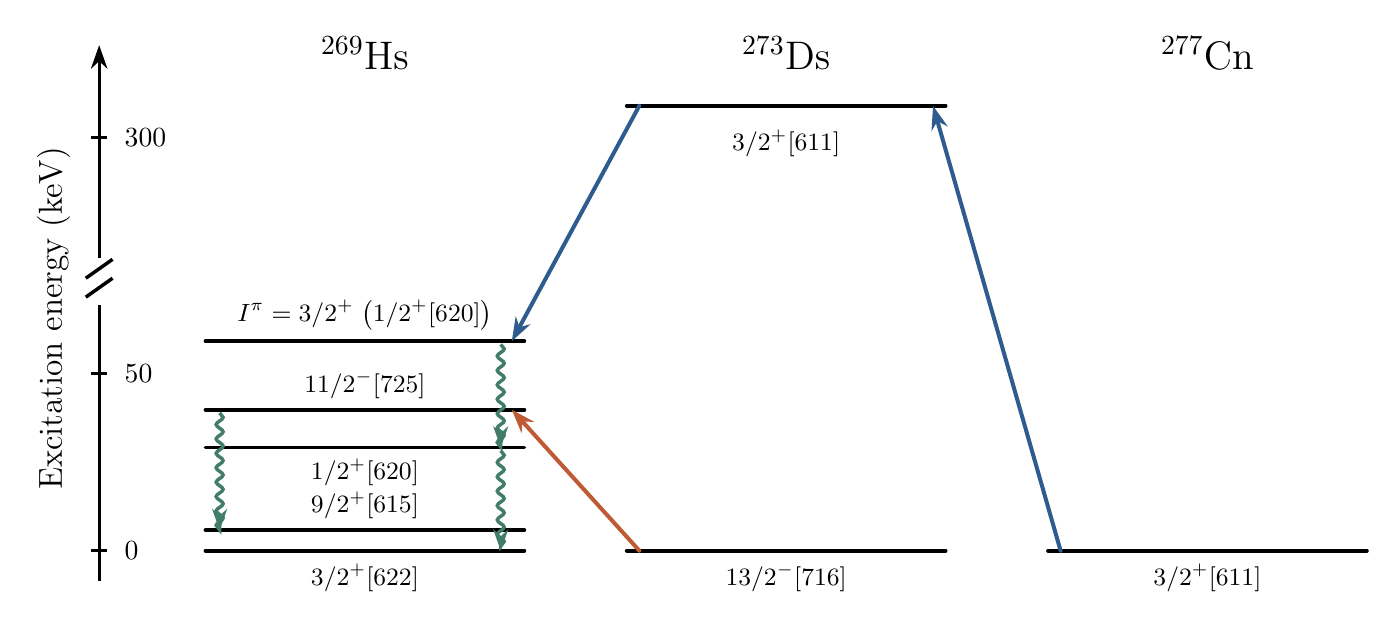
\begin{tikzpicture}[
    x=1cm,
    y=1cm,
    level/.style={
        line width=1.35pt,
        line cap=round
    },
    transition/.style={
        -{Stealth[length=3.0mm,width=2.1mm]},
        line width=1.45pt,
        line cap=round
    },
    gamma/.style={
        decorate,
        decoration={
            snake,
            amplitude=1.25pt,
            segment length=5.2pt
        },
        -{Stealth[length=2.7mm,width=1.9mm]},
        line width=1.25pt
    },
    state/.style={
        font=\small,
        inner sep=1pt
    },
    nucleus/.style={
        font=\Large\bfseries
    },
    ticklabel/.style={
        font=\normalsize
    }
]

% ============================================================
% Muted scientific colors
% ============================================================

\definecolor{branchblue}{RGB}{47,92,143}
\definecolor{branchorange}{RGB}{190,91,52}
\definecolor{gammagreen}{RGB}{66,125,103}

% ============================================================
% Common vertical coordinates
% ============================================================

% Ground-state reference
\def\yZero{1.20}

% 269Hs states, including the I=1/2+ bandhead and its
% higher-lying I=3/2+ rotational-band member.
\def\yHsFive{1.46}       % 5.8 keV
\def\yHsBandHead{2.51}   % 29.2-keV 1/2+[620] bandhead
\def\yHsLong{2.99}       % 39.7-keV 11/2-[725] state
\def\yHsBandThree{3.86}  % 59.2-keV I=3/2+ band member

% Axis reference ticks
\def\yFifty{3.45}        % 50 keV
\def\yThreeHundred{6.45} % 300 keV

% Broken-axis positions
\def\yBreakLow{4.32}
\def\yBreakHigh{4.92}

% 273Ds first excited state
\def\yDsExcited{6.85}    % approximately 320 keV

% ============================================================
% Horizontal coordinates: from right to left, 277Cn -> 273Ds -> 269Hs
% ============================================================

\def\xAxis{-0.35}

\def\xHsL{1.00}
\def\xHsR{5.05}

\def\xDsL{6.35}
\def\xDsR{10.40}

\def\xCnL{11.70}
\def\xCnR{15.75}

% ============================================================
% Excitation-energy axis
% ============================================================

% Lower continuous section
\draw[line width=1.05pt]
    (\xAxis,0.82)
    --
    (\xAxis,\yBreakLow);

% Upper continuous section
\draw[line width=1.05pt]
    (\xAxis,\yBreakHigh)
    --
    (\xAxis,7.25);

% Arrow at the top of the axis
\draw[
    -{Stealth[length=3.0mm,width=2.1mm]},
    line width=1.05pt
]
    (\xAxis,7.25)
    --
    (\xAxis,7.62);

% Axis ticks and labels
\draw[line width=1.0pt]
    (\xAxis-0.10,\yZero)
    --
    (\xAxis+0.10,\yZero);

\node[ticklabel,anchor=west]
    at (\xAxis+0.20,\yZero)
    {$0$};

\draw[line width=1.0pt]
    (\xAxis-0.10,\yFifty)
    --
    (\xAxis+0.10,\yFifty);

\node[ticklabel,anchor=west]
    at (\xAxis+0.20,\yFifty)
    {$50$};

\draw[line width=1.0pt]
    (\xAxis-0.10,\yThreeHundred)
    --
    (\xAxis+0.10,\yThreeHundred);

\node[ticklabel,anchor=west]
    at (\xAxis+0.20,\yThreeHundred)
    {$300$};

% Double-slash break
\draw[line width=1.25pt]
    (\xAxis-0.17,4.42)
    --
    (\xAxis+0.17,4.66);

\draw[line width=1.25pt]
    (\xAxis-0.17,4.66)
    --
    (\xAxis+0.17,4.90);

\node[font=\large,rotate=90]
    at (\xAxis-0.58,4.15)
    {Excitation energy (keV)};

% ============================================================
% Nucleus labels
% ============================================================

\node[nucleus]
    at ({(\xHsL+\xHsR)/2},7.52)
    {$^{269}\mathrm{Hs}$};

\node[nucleus]
    at ({(\xDsL+\xDsR)/2},7.52)
    {$^{273}\mathrm{Ds}$};

\node[nucleus]
    at ({(\xCnL+\xCnR)/2},7.52)
    {$^{277}\mathrm{Cn}$};

% ============================================================
% 269Hs levels
% ============================================================

% Ground state
\draw[level]
    (\xHsL,\yZero)
    --
    (\xHsR,\yZero);

\node[state,anchor=north]
    at ({(\xHsL+\xHsR)/2},\yZero-0.13)
    {$3/2^{+}[622]$};

% 5.8-keV state
\draw[level]
    (\xHsL,\yHsFive)
    --
    (\xHsR,\yHsFive);

\node[state,anchor=south]
    at ({(\xHsL+\xHsR)/2},\yHsFive+0.10)
    {$9/2^{+}[615]$};

% 1/2+[620] rotational-band head
\draw[level]
    (\xHsL,\yHsBandHead)
    --
    (\xHsR,\yHsBandHead);

\node[state,anchor=north]
    at ({(\xHsL+\xHsR)/2},\yHsBandHead-0.10)
    {$1/2^{+}[620]$};

% 39.7-keV state used by the long-lived branch
\draw[level]
    (\xHsL,\yHsLong)
    --
    (\xHsR,\yHsLong);

\node[state,anchor=south]
    at ({(\xHsL+\xHsR)/2},\yHsLong+0.10)
    {$11/2^{-}[725]$};

% I=3/2+ member of the 1/2+[620] rotational band
\draw[level]
    (\xHsL,\yHsBandThree)
    --
    (\xHsR,\yHsBandThree);

\node[state,anchor=south]
    at ({(\xHsL+\xHsR)/2},\yHsBandThree+0.10)
    {$I^{\pi}=3/2^{+}\;\bigl(1/2^{+}[620]\bigr)$};

% ============================================================
% 273Ds levels
% ============================================================

% Ground state
\draw[level]
    (\xDsL,\yZero)
    --
    (\xDsR,\yZero);

\node[state,anchor=north]
    at ({(\xDsL+\xDsR)/2},\yZero-0.13)
    {$13/2^{-}[716]$};

% First excited state
\draw[level]
    (\xDsL,\yDsExcited)
    --
    (\xDsR,\yDsExcited);

\node[state,anchor=north]
    at ({(\xDsL+\xDsR)/2},\yDsExcited-0.26)
    {$3/2^{+}[611]$};

% ============================================================
% 277Cn level
% ============================================================

% Ground state
\draw[level]
    (\xCnL,\yZero)
    --
    (\xCnR,\yZero);

\node[state,anchor=north]
    at ({(\xCnL+\xCnR)/2},\yZero-0.13)
    {$3/2^{+}[611]$};

% ============================================================
% Alpha-decay branches, directed from right to left
% ============================================================

% 277Cn ground state -> 273Ds 3/2+[611]
\draw[
    transition,
    branchblue
]
    (\xCnL+0.16,\yZero)
    --
    (\xDsR-0.16,\yDsExcited);

% 273Ds 3/2+[611] -> I=3/2+ member of the 1/2+[620] band
\draw[
    transition,
    branchblue
]
    (\xDsL+0.16,\yDsExcited)
    --
    (\xHsR-0.16,\yHsBandThree);

% 273Ds 13/2-[716] -> 269Hs 11/2-[725]
\draw[
    transition,
    branchorange
]
    (\xDsL+0.16,\yZero)
    --
    (\xHsR-0.16,\yHsLong);

% ============================================================
% Gamma de-excitation in 269Hs
% ============================================================

% 11/2-[725] -> 9/2+[615]
\draw[
    gamma,
    gammagreen
]
    (\xHsL+0.18,\yHsLong-0.04)
    --
    (\xHsL+0.18,\yHsFive);

% I=3/2+ -> I=1/2+ within the 1/2+[620] rotational band
\draw[
    gamma,
    gammagreen
]
    (\xHsR-0.30,\yHsBandThree-0.04)
    --
    (\xHsR-0.30,\yHsBandHead);

% 1/2+[620] bandhead -> 3/2+[622] ground state
\draw[
    gamma,
    gammagreen
]
    (\xHsR-0.30,\yHsBandHead-0.04)
    --
    (\xHsR-0.30,\yZero);

\end{tikzpicture}

\end{document}
